\section{Experimental anomalies beyond the PMNS framework}
\label{sec:anomalies}

The vast majority of experimental measurement related to neutrino oscillations can be described in the framework of the PMNS matrix as reported in the previous sections. There are however some unresolved anomalies: 
\begin{itemize}
\item The LSND experiment~\cite{lsnd} reported an excess of $87.9 \pm 22.4 \pm 6.0$ events consistent with $\bar{\nu}_e p \rightarrow e^+ n$ scattering while studying $\bar{\nu}_\mu$ (endpoint energy 52 MeV) from $\mu^+$ decaying at rest, with a distance from the source to the liquid scintillator detector (167 tons) of 30~m. This might be interpreted as evidence for $\bar{\nu}_\mu \rightarrow  \bar{\nu}_e$ neutrino oscillations with $\Delta m^2$ in the 0.2-10 eV$^2$/c$^2$ range.
\item The MiniBooNE~\cite{miniboone1,miniboone2} experiment was built to confirm the LSND claim with a muon neutrino beam at FNAL, whose peak energy is 600 MeV for neutrinos and 400 MeV for antineutrinos. It consists of a tank containing 806 tons of mineral oil equipped with 1520 PMTs at 540~m from the beam target. It reported unexplained excesses in the low-energy region of electron neutrinos (162.0 $\pm$ 47.8 events) and antineutrinos (78.4 $\pm$ 28.5 events) at the 3.4 and 2.8 $\sigma$ levels. The energy distribution of the excess in the neutrino channel is only marginally compatible within a simple two-neutrinos effective framework. 
\item The GALLEX and SAGE Gallium solar neutrino experiments have been calibrated using intense radioactive sources ($^{51}$Cr and $^{37}$Ar) placed inside the detectors~\cite{gallium}. The measured event rate is lower than expected, with the ratio of observed over expected rate $0.86\pm 0.05$ deviating from 1 at the 2.8 $ \sigma$ level. This constitutes the Gallium anomaly. 
\item A recent re-evaluation~\cite{mueller} of the reactor neutrino flux combining an {\it ab initio} calculation of the spectrum related to $^{238} U$ and a revised $\beta$ inversion method for the other actinides resulted in an upward shift of the normalization by 3\% on average. A comparison of the expected with the observed antineutrino rate in short-baseline reactor experiments (L $< 100 m$ and down to 9 m for the ILL experiment and 15 m for the Bugey-4 experiment) results in a ratio of $ 0.943 \pm 0.023$~\cite{mention}. This constitutes the reactor anomaly. 
\end{itemize}

All these anomalies can be interpreted as hinting to the existence of oscillation of active neutrinos towards a sterile state with a $\Delta m^2$ around 1 eV$^2$/c$^2$. 
It must be stressed that, while all the measurements related to the various sectors of the PMNS matrix have been confirmed by several experiments with very different techniques (for instance the $ \theta_{23}$ oscillations have been observed by experiments using atmospheric neutrinos and by long baseline experiments), each of this anomaly is rather isolated. Moreover, the statistical significance is far from being compelling and does not exceed 3 $\sigma$. 
Repeated and numerous attempts have been made to interpret these anomalies in models where the three known active neutrinos mix with a fourth sterile state (3+1) or with two new sterile states (3+2).
 In the 3+1 model, in the limit where the phases relative to $\Delta m^2_{21}$ and $\Delta m^2_{31}$ can be neglected  the survival probability reads
\begin{equation}
P(\nu_e \rightarrow \nu_e) = 1 - 4 |U_{e4}|^2 (1 - 4 |U_{e4}|^2) \sin^2 \frac{\Delta m^2_{41}L}{4E} = 1 - \sin^2 2\theta_{ee} \sin^2 \frac{\Delta m^2_{41}L}{4E}
\end{equation}
where the effective mixing angle $\theta_{ee}$ is defined as $\sin^2 2 \theta_{ee} = 4 |U_{e4}|^2 (1 - 4 |U_{e4}|^2)$. 

To interpret the results of the LSND and MiniBooNE experiments both the $U_{e4}$ and the $U_{\mu 4}$ matrix elements should be different from zero and the appearance probability reads
\begin{equation}
P(\nu_\mu \rightarrow \nu_e) = |U_{e4} U_{\mu 4}|^2  \sin^2 \frac{\Delta m^2_{41}L}{4E} = \sin^2 2 \theta_{\mu e} \sin^2 \frac{\Delta m^2_{41}L}{4E}
\end{equation}
with $\sin^2 2 \theta_{\mu e} = 4 |U_{e4} U_{\mu 4}|^2$.
The formulae are more complex in 3+2 models, where the number of free parameters of the models is larger.

Global fits to the world dataset corresponding to these anomalies and all other experimental results on neutrino oscillations measurements and searches have been attempted \cite{giuntirev,kopp}. The result is that there is a strong tension between appearance experiments like LSND and MiniBooNE and the negative results from disappearance experiments like CDHS~\cite{dydak}. Oscillations in the $\bar{\nu}_\mu \rightarrow  \bar{\nu}_e$ channels inevitably entail disappearance in the 
$\bar{\nu}_\mu \rightarrow  \bar{\nu}_\mu$ channel with the same L/E range. This disappearance has not been observed. The compatibility of appearance and disappearance data is at the level of $10^{-4}$ for 3+1 models~\cite{kopp}. More complex models like 3+2 do not alleviate this tension. 

\begin{figure}[htbp]
\begin{minipage}[c]{.46\linewidth}
%\begin{minipage}[c]
   	      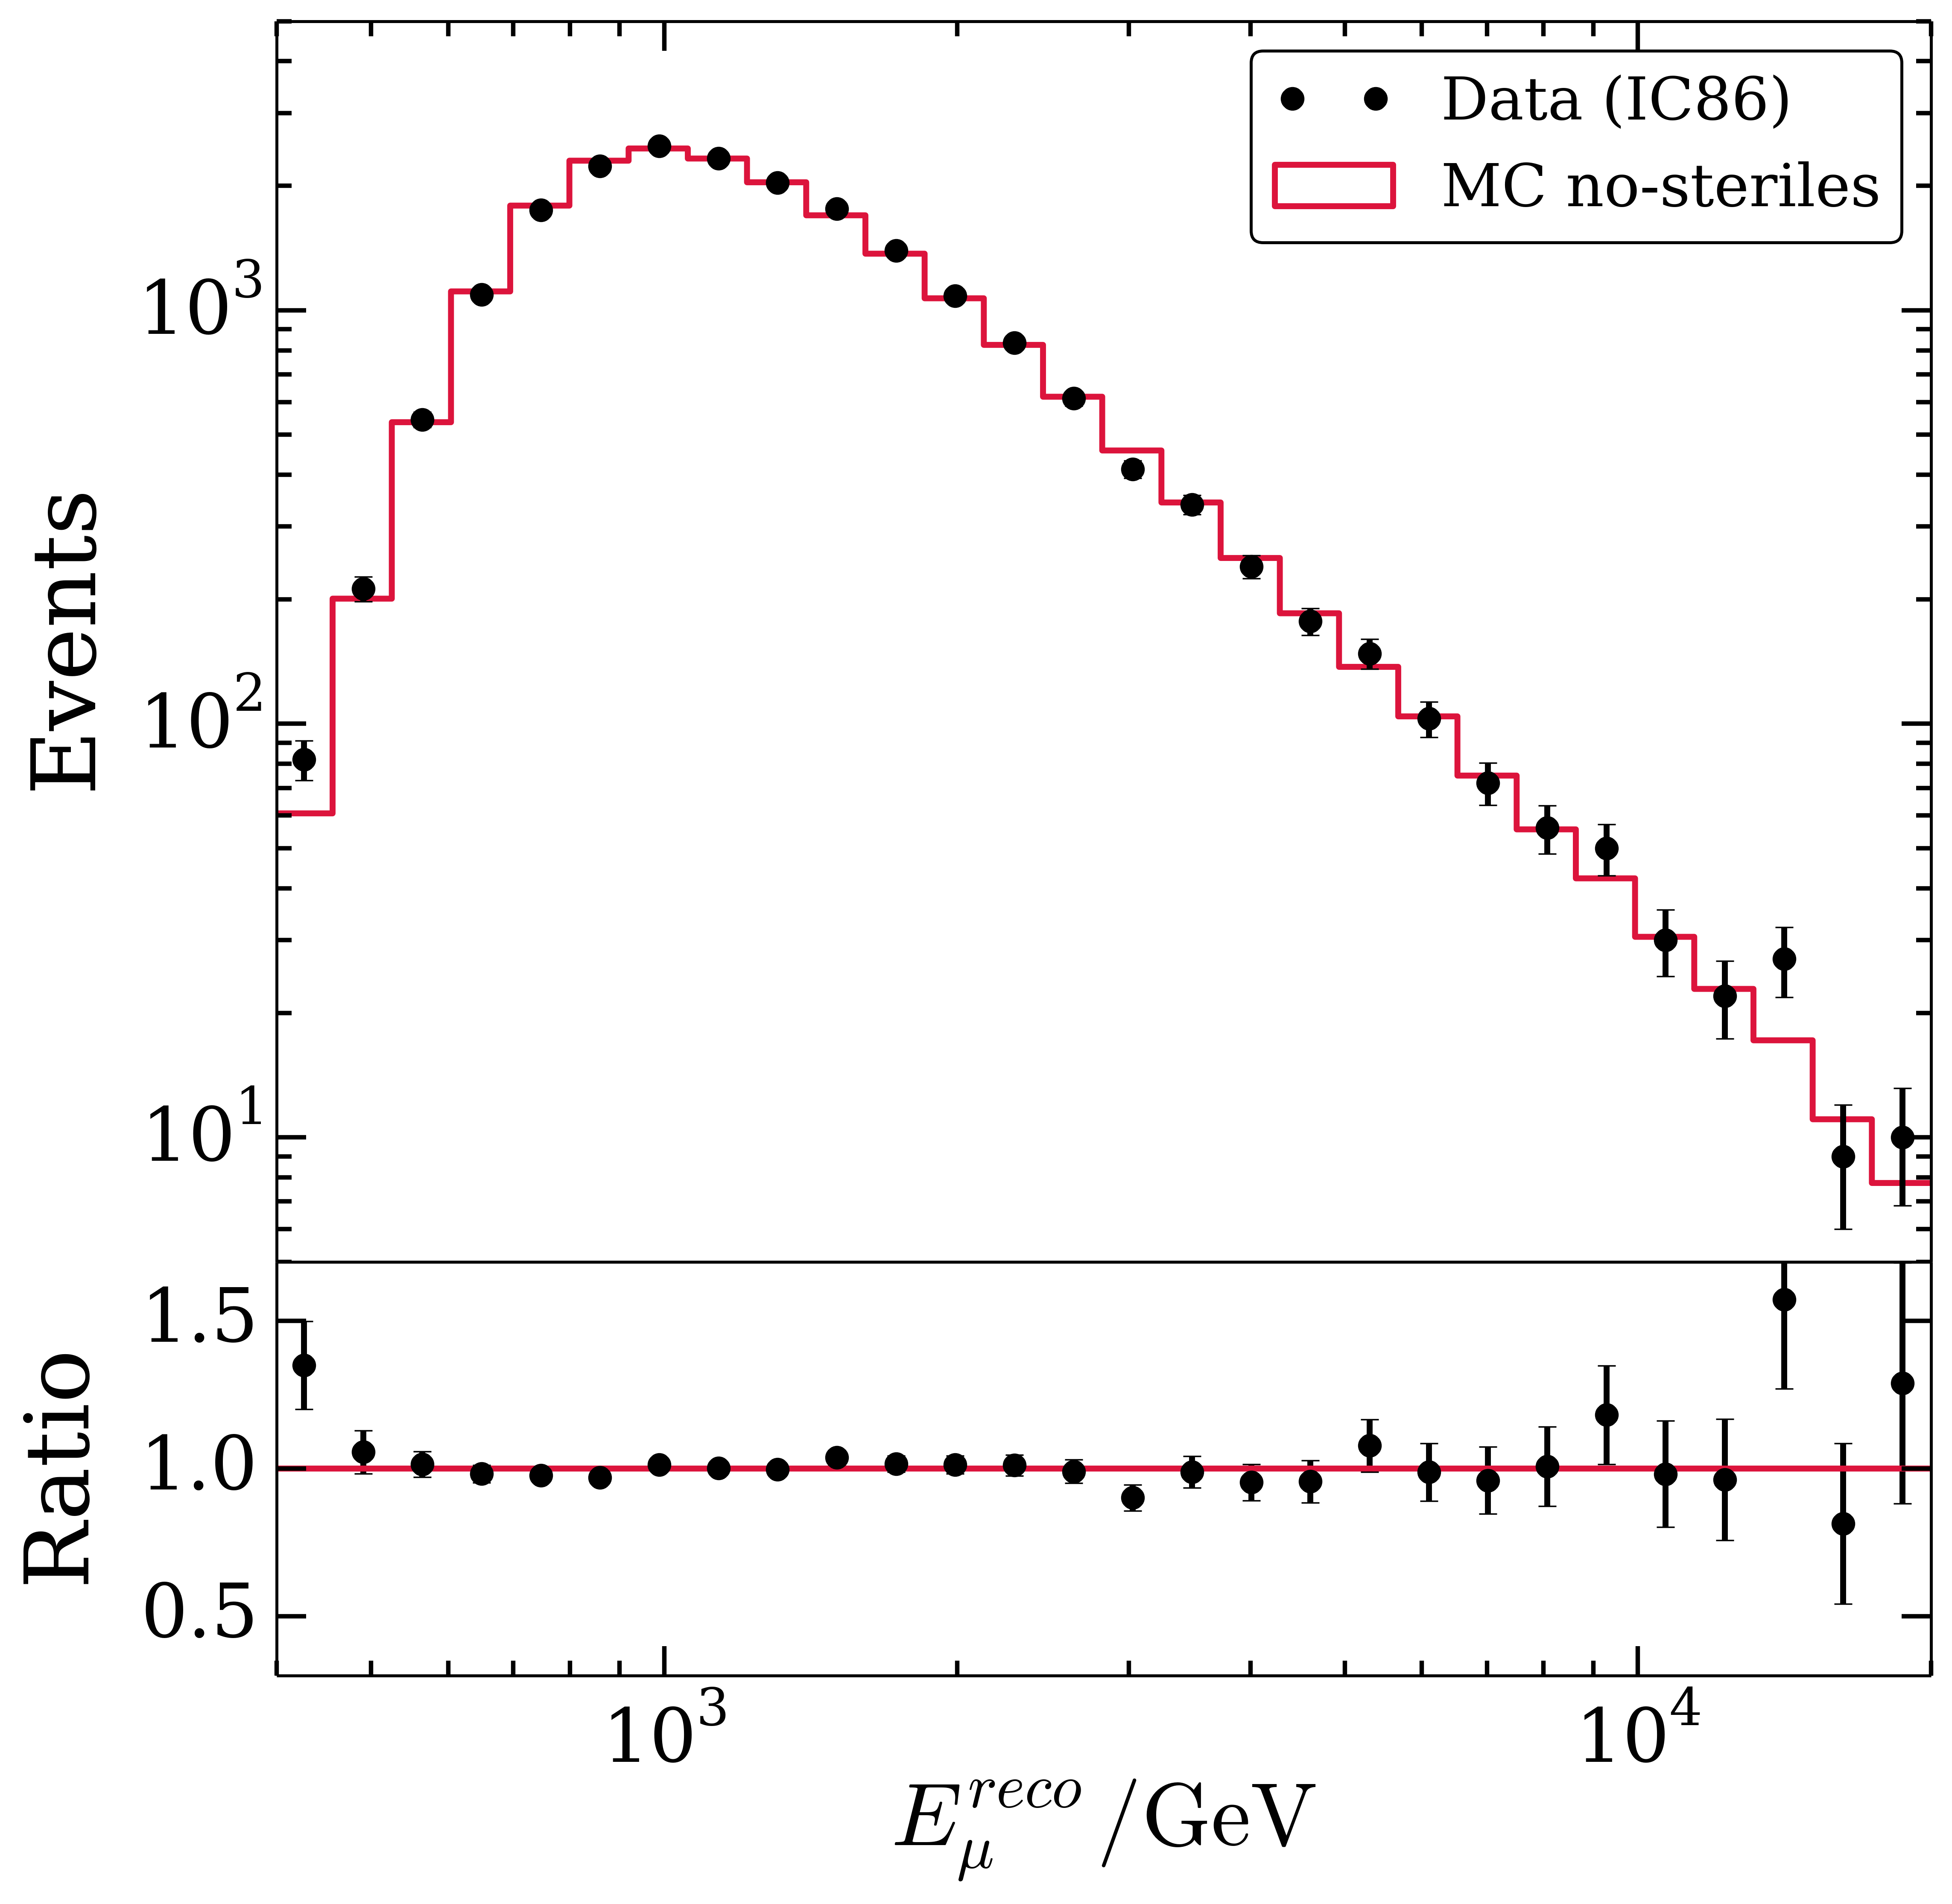
\includegraphics[width=0.9\linewidth]{figures/EnergyDist-2.png}
   \end{minipage} \hfill
   \begin{minipage}{.46\linewidth}
      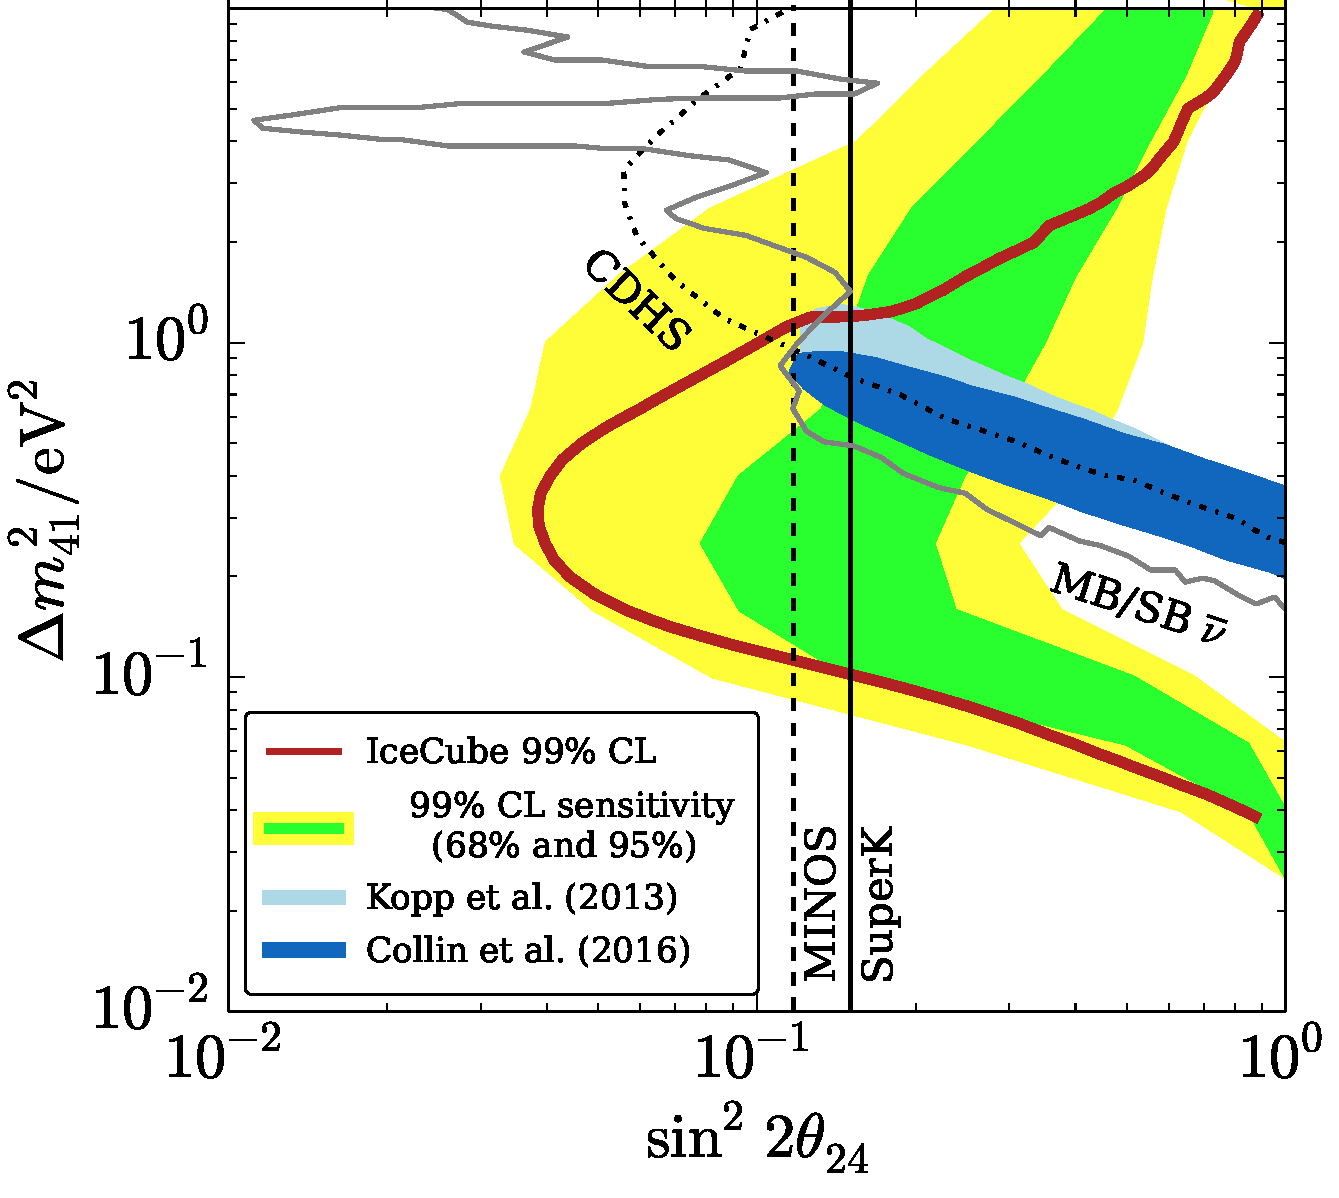
\includegraphics[width=0.9\linewidth]{figures/icecube-sterile-crop.pdf}
   \end{minipage}
    \caption{The reconstructed energy distribution of atmospheric $\nu_\mu$ events observed by the IceCube experiment compared to the prediction without sterile neutrinos (left). 
The 99%
(red solid line) CL contour in the $\Delta m^2_{41}$ versus $\sin² (2 \theta_{24}$ obtained by the IceCube experiment is shown with bands containing
68\% (green) and 95\% (yellow) of the 99\% contours in sim-
ulated pseudo-experiments, respectively. The contours and
bands are overlaid on 90\% CL exclusions from previous experiments [7–10], and the MiniBooNE / LSND 90\% CL allowed
region from [12, 13, 21] assuming $|U_{e4}|^2 = 0.023$.  }
 \label{fig:icecube-sterile}
\end{figure}

Very recent data instead of confirming this picture actually bring more experimental evidence against the LSND and MiniBooNE anomalies.
The IceCube has studied the atmospheric muon neutrino spectrum in the energy range 320 GeV to 20 TeV~\cite{icecubeste}. Muon neutrino mixing with a sterile state with $\Delta m^2_{41}$ in the 1 eV$^2$ range would strongly deplete the observed antineutrino spectrum for 3+1 models mainly due to MSW resonance effects during neutrino propagation in the Earth. The deficit can reach 11\% for the bin with the largest effect in the distribution of reconstructed energy and zenith angle. Similar effects would deplete the neutrino spectrum for 1+3 models. No depletion is observed in a sample of 20145 well reconstructed muons registered with an 86 strings configuration in 2011 and 2012. They set strong limits in the 
$\Delta m^2_{41}$ versus $\sin² (2 \theta_{24}$ plane. The allowed region from the appearance experiments LSND and MiniBooNE is excluded at the 99\% CL (Fig.~\ref{fig:icecube-sterile}).  

An interesting limit has been set by a combined analysis of the MINOS, Daya Bay and Bugey-3 data. MINOS is sensitive to a sterile neutrino as active (mainly $\nu_\mu$ in this case)-sterile mixing would modify the shape and normalization of charged current and neutral current events in the near and far detectors.
It can therefore set limits on $|U_{\mu 4}|^2$. Bugey-3 and Daya Bay data can be used to constrain electron antineutrino disappearance and place limits on $|U_{e 4}|^2$. The combination of these three experiments excludes the phase space allowed by the LSND and MiniBooNE experiments below 0.8 eV$^2$ at 95 \% CL~\cite{dayabaycomb}. 

The reactor and Gallium anomalies are not in such a conflict with other measurements. In this sector, recent developments have focussed on the reliability of systematic uncertainty related to the understanding of the reactor antineutrino flux. The observation of the 5 MeV bump has indeed brought under close scrutiny the method to compute the reactor antineutrino flux. The conclusions of recent studies \cite{hayes,vogel} are that several uncertainties might have been underestimated. For instance, 30\% of the flux comes from forbidden transitions. The effect of various shape corrections applied to forbidden transitions has been investigated and it leads to a 4-5\% uncertainty on the reactor antineutrino flux. Taking into account this uncertainty would considerably release the tension at the origin of the reactor anomaly.

A new generation of reactor neutrino experiments (STEREO, SOLID, NEUTRINO-4, DANSS, NEOS, see \cite{othervsbl} for a review) has been built to investigate in detail the possible mixing of $\nu_e$ with a sterile state with $\Delta m^2_{41}$ in the 1 eV$^2$/c$^2$ range.
Indeed $\bar{\nu}_e \rightarrow \nu_s$ oscillations would induce a deformation of the spectrum if the detector is placed close enough (L$\simeq$ 10m) to the reactor core. Several of these experiments will take data starting in 2017 or earlier and so new results on this hot topic are expected soon.
The SOX experiment \cite{cribier} will deploy an intense $^{144}$Ce antineutrino source very close to the Borexino detector with data taking in 2018.

The three Liquid Argon detectors complex SBN \cite{sbnfnal} is in construction at FNAL. The 170 t MicroBooNE Liquid Argon detector has been built on the Booster Neutrino beam, the same beam used by MiniBooNE, at L=470m from the target. It will be completed by the refurbished ICARUS detector (760 t) placed at 600~m and by the LAr1-ND near detector (220 t)  at 110~m from the production target, for the investigation of these anomalies both in the appearance and in the disappearance channels. This set of detectors will be able to probe the LSND appearance excess with a sensitivity of 5 $\sigma$. The installation will be completed in 2018.    

